\documentclass[11pt,a4paper]{report}
\usepackage[textwidth=37em,vmargin=30mm]{geometry}
\usepackage{calc,xunicode,amsmath,amssymb,paralist,enumitem,tabu,booktabs,datetime2,xeCJK,xeCJKfntef,listings}
\usepackage{tocloft,fancyhdr,tcolorbox,xcolor,graphicx,eso-pic,xltxtra,xelatexemoji}

\newcommand{\envyear}[0]{2024}
\newcommand{\envdatestr}[0]{2024-11-21}
\newcommand{\envfinaldir}[0]{webdb/2024/20241121/final}

\usepackage[hidelinks]{hyperref}
\hypersetup{
    colorlinks=false,
    pdfpagemode=FullScreen,
    pdftitle={Web Digest - \envdatestr}
}

\setlength{\cftbeforechapskip}{10pt}
\renewcommand{\cftchapfont}{\rmfamily\bfseries\large\raggedright}
\setlength{\cftbeforesecskip}{2pt}
\renewcommand{\cftsecfont}{\sffamily\small\raggedright}

\setdefaultleftmargin{2em}{2em}{1em}{1em}{1em}{1em}

\usepackage{xeCJK,xeCJKfntef}
\xeCJKsetup{PunctStyle=plain,RubberPunctSkip=false,CJKglue=\strut\hskip 0pt plus 0.1em minus 0.05em,CJKecglue=\strut\hskip 0.22em plus 0.2em}
\XeTeXlinebreaklocale "zh"
\XeTeXlinebreakskip = 0pt


\setmainfont{Brygada 1918}
\setromanfont{Brygada 1918}
\setsansfont{IBM Plex Sans}
\setmonofont{JetBrains Mono NL}
\setCJKmainfont{Noto Serif CJK SC}
\setCJKromanfont{Noto Serif CJK SC}
\setCJKsansfont{Noto Sans CJK SC}
\setCJKmonofont{Noto Sans CJK SC}

\setlength{\parindent}{0pt}
\setlength{\parskip}{8pt}
\linespread{1.15}

\lstset{
	basicstyle=\ttfamily\footnotesize,
	numbersep=5pt,
	backgroundcolor=\color{black!5},
	showspaces=false,
	showstringspaces=false,
	showtabs=false,
	tabsize=2,
	captionpos=b,
	breaklines=true,
	breakatwhitespace=true,
	breakautoindent=true,
	linewidth=\textwidth
}






\newcommand{\coverpic}[2]{
    % argv: itemurl, authorname
    Cover photo by #2~~(\href{#1}{#1})
}
\newcommand{\makeheader}[0]{
    \begin{titlepage}
        % \newgeometry{hmargin=15mm,tmargin=21mm,bmargin=12mm}
        \begin{center}
            
            \rmfamily\scshape
            \fontspec{BaskervilleF}
            \fontspec{Old Standard}
            \fontsize{59pt}{70pt}\selectfont
            WEB\hfill DIGEST
            
            \vfill
            % \vskip 30pt
            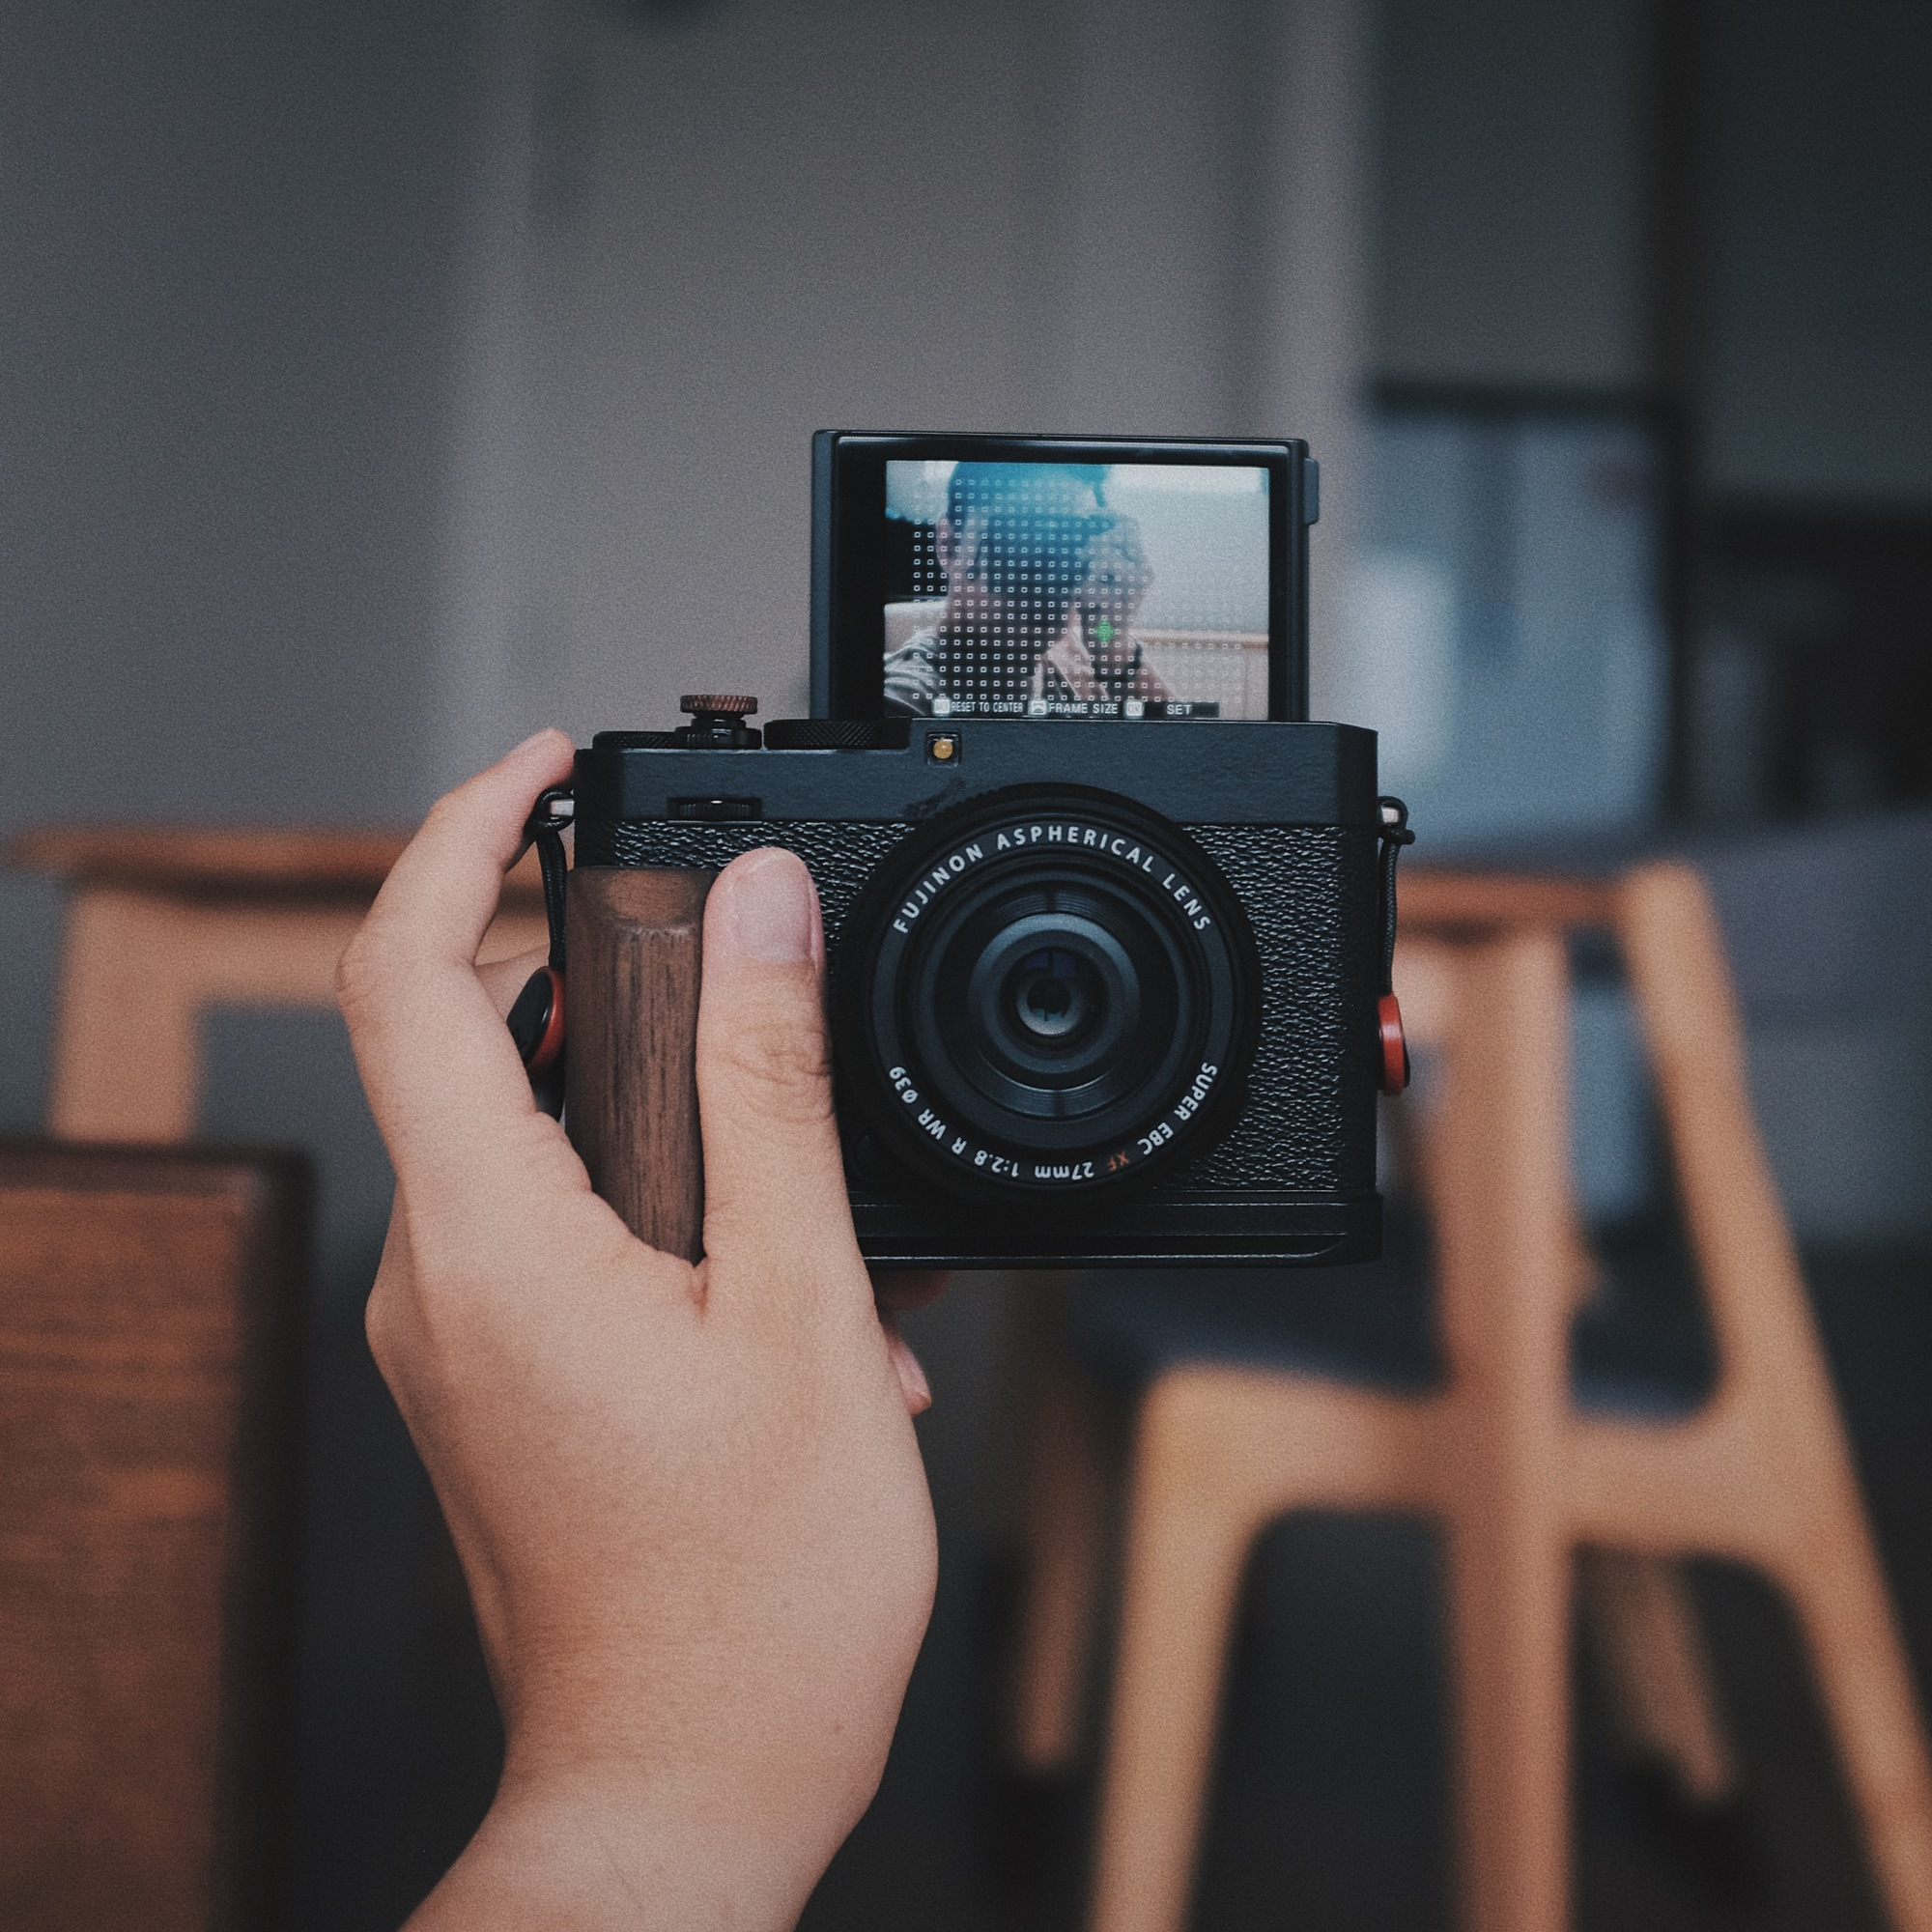
\includegraphics[width=\linewidth]{\envfinaldir/coverpic-prod.jpg}\par
            % \vskip 30pt
            \vfill

            \normalsize\rmfamily\scshape
            \copyright{} The Web Digest Project \hfill\large \envdatestr
        \end{center}
    \end{titlepage}
    % \restoregeometry
}
\newcommand{\simplehref}[1]{%
    \textcolor{blue!80!green}{\href{#1}{#1}}%
}
\renewcommand{\contentsname}{\center\Huge\sffamily\bfseries Contents\par\vskip 20pt}
\newcounter{ipartcounter}
\setcounter{ipartcounter}{0}
\newcommand{\ipart}[1]{
    % \vskip 20pt
    \clearpage
    \stepcounter{ipartcounter}
    \phantomsection
    \addcontentsline{toc}{chapter}{#1}
    % \begin{center}
    %     \Huge
    %     \sffamily\bfseries
    %     #1
    % \end{center}
    % \vskip 20pt plus 7pt
}
\newcounter{ichaptercounter}
\setcounter{ichaptercounter}{0}
\newcommand{\ichapter}[1]{
    % \vskip 20pt
    \clearpage
    \stepcounter{ichaptercounter}
    \phantomsection
    \addcontentsline{toc}{section}{\numberline{\arabic{ichaptercounter}}#1}
    \begin{center}
        \Huge
        \sffamily\bfseries
        #1
    \end{center}
    \vskip 20pt plus 7pt
}
\newcommand{\entrytitlefont}[1]{\subsection*{\raggedright\Large\sffamily\bfseries#1}}
\newcommand{\entryitemGeneric}[2]{
    % argv: title, url
    \parbox{\linewidth}{
        \entrytitlefont{#1}\par\vskip 5pt
        \footnotesize\ttfamily\mdseries
        \simplehref{#2}
    }\vskip 11pt plus 11pt minus 1pt
}
\newcommand{\entryitemGithub}[3]{
    % argv: title, url, desc
    \parbox{\linewidth}{
        \entrytitlefont{#1}\par\vskip 5pt
        \footnotesize\ttfamily\mdseries
        \simplehref{#2}\par\vskip 5pt
        \small\rmfamily\mdseries#3
    }\vskip 11pt plus 11pt minus 1pt
}
\newcommand{\entryitemAp}[3]{
    % argv: title, url, desc
    \parbox{\linewidth}{
        \entrytitlefont{#1}\par\vskip 5pt
        \footnotesize\ttfamily\mdseries
        \simplehref{#2}\par\vskip 5pt
        \small\rmfamily\mdseries#3
    }\vskip 11pt plus 11pt minus 1pt
}
\newcommand{\entryitemHackernews}[3]{
    % argv: title, hnurl, rawurl
    % \parbox{\linewidth}{
    %     \entrytitlefont{#1}\par\vskip 5pt
    %     \footnotesize\ttfamily\mdseries
    %     \simplehref{#3}\par
    %     \textcolor{black!50}{\href{#2}{#2}}
    % }\vskip 11pt plus 11pt minus 1pt
    \begin{minipage}{\linewidth}
            \entrytitlefont{#1}\par\vskip 5pt
            \footnotesize\ttfamily\mdseries
            \simplehref{#3}\par
            \textcolor{black!50}{\href{#2}{#2}}
    \end{minipage}\par\vskip 11pt plus 11pt minus 1pt
}







\begin{document}

\makeheader

\tableofcontents\clearpage




\ipart{Developers}
\ichapter{Hacker News}
\entryitemTwoLinks{SQL, Homomorphisms and Constraint Satisfaction Problems}{https://news.ycombinator.com/item?id=42195994}{https://www.philipzucker.com/sql\_graph\_csp/}

\entryitemTwoLinks{Undergraduates with family income below \$200k will be tuition-free at MIT}{https://news.ycombinator.com/item?id=42195895}{https://news.mit.edu/2024/mit-tuition-undergraduates-family-income-1120}

\entryitemTwoLinks{La Basilica Di San Pietro}{https://news.ycombinator.com/item?id=42194587}{https://unlocked.microsoft.com/vatican/}

\entryitemTwoLinks{How good are American roads?}{https://news.ycombinator.com/item?id=42194327}{https://www.construction-physics.com/p/how-good-are-american-roads}

\entryitemTwoLinks{GNU Artanis 1.0.0 Released}{https://news.ycombinator.com/item?id=42194315}{https://artanis.dev/blog/1.0.0-release.html}

\entryitemTwoLinks{What is the origin of the lake tank image that has become a meme? (2021)}{https://news.ycombinator.com/item?id=42193771}{https://history.stackexchange.com/questions/57033/what-is-the-origin-of-the-lake-tank-image-that-has-become-a-meme}

\entryitemTwoLinks{Bluesky is ushering in a pick-your-own algorithm era of social media}{https://news.ycombinator.com/item?id=42193549}{https://www.newscientist.com/article/2456782-bluesky-is-ushering-in-a-pick-your-own-algorithm-era-of-social-media/}

\entryitemTwoLinks{Why don't you move abroad?}{https://news.ycombinator.com/item?id=42191805}{https://orkohunter.net/blog/why-dont-you-move-abroad/}

\entryitemTwoLinks{Foursquare Open Source Places: A new foundational dataset}{https://news.ycombinator.com/item?id=42191781}{https://simonwillison.net/2024/Nov/20/foursquare-open-source-places/}

\entryitemTwoLinks{AAA – Analytical Anti-Aliasing}{https://news.ycombinator.com/item?id=42191709}{https://blog.frost.kiwi/analytical-anti-aliasing/}

\entryitemTwoLinks{Yi Peng 3 crossed both cables C-Lion 1 and BSC at times matching when they broke}{https://news.ycombinator.com/item?id=42191394}{https://bsky.app/profile/auonsson.bsky.social/post/3lbc5va7f722p}

\entryitemTwoLinks{Lush: My favorite small programming language}{https://news.ycombinator.com/item?id=42191354}{https://scottlocklin.wordpress.com/2024/11/19/lush-my-favorite-small-programming-language/}

\entryitemTwoLinks{Let's Encrypt is 10 years old now}{https://news.ycombinator.com/item?id=42191228}{https://letsencrypt.org/2014/11/18/announcing-lets-encrypt/}

\entryitemTwoLinks{Blender 4.3}{https://news.ycombinator.com/item?id=42190863}{https://www.blender.org/download/releases/4-3/}

\entryitemTwoLinks{Understanding the BM25 full text search algorithm}{https://news.ycombinator.com/item?id=42190650}{https://emschwartz.me/understanding-the-bm25-full-text-search-algorithm/}

\entryitemTwoLinks{Epic Allows Internet Archive to Distribute Unreal and Unreal Tournament Forever}{https://news.ycombinator.com/item?id=42190541}{https://www.techdirt.com/2024/11/18/epic-allows-internet-archive-to-distribute-for-free-unreal-unreal-tournament-forever/}

\entryitemTwoLinks{Webvm: Virtual Machine for the Web}{https://news.ycombinator.com/item?id=42190395}{https://github.com/leaningtech/webvm}

\entryitemTwoLinks{Tiny Glade 'built' its way to >600k sold in a month}{https://news.ycombinator.com/item?id=42190065}{https://newsletter.gamediscover.co/p/how-tiny-glade-built-its-way-to-600k}

\entryitemTwoLinks{Meta Uses LLMs to Improve Incident Response}{https://news.ycombinator.com/item?id=42189991}{https://www.tryparity.com/blog/how-meta-uses-llms-to-improve-incident-response}

\entryitemTwoLinks{Ask HN: Bluesky Accounts Worth Following for HN Enthusiasts}{https://news.ycombinator.com/item?id=42189890}{https://news.ycombinator.com/item?id=42189890}\ichapter{Phoronix}
\entryitemGeneric{\hskip 0pt{}Linux 6.13 "MM" Patches Bring Some Enticing Performance Optimizations}{https://www.phoronix.com/news/Linux-6.13-MM-Patches}

\entryitemGeneric{\hskip 0pt{}Many Networking Changes In Linux 6.13 - One Line Of Code Helping WireGuard Performance}{https://www.phoronix.com/news/Linux-6.13-Networking}

\entryitemGeneric{\hskip 0pt{}8 vs. 12 Channel DDR5-6000 Memory Performance With AMD 5th Gen EPYC}{https://www.phoronix.com/review/8-12-channel-epyc-9005}

\entryitemGeneric{\hskip 0pt{}Raspberry Pi Camera Front End "CFE" Video Capture With Linux 6.13}{https://www.phoronix.com/news/Raspberry-Pi-CFE-Linux-6.13}

\entryitemGeneric{\hskip 0pt{}Many AMD CPU Feature Additions Land In Linux 6.13}{https://www.phoronix.com/news/Linux-6.13-AMD-CPU}

\entryitemGeneric{\hskip 0pt{}OpenVINO 2024.5 Released With More Intel Optimizations, Better LLM/GenAI Coverage}{https://www.phoronix.com/news/OpenVINO-2024.5-Released}

\entryitemGeneric{\hskip 0pt{}Faster CRC32C \& AEGIS-128 Crypto Performance On Linux 6.13 With Intel/AMD CPUs}{https://www.phoronix.com/news/Linux-6.13-Crypto}

\entryitemGeneric{\hskip 0pt{}Multigrain Timestamps Try Again For Linux 6.13 - Now With Less Performance Impact}{https://www.phoronix.com/news/Linux-6.13-Multigrain-Timestamp}

\entryitemGeneric{\hskip 0pt{}Corsair Void Headset \& Kysona M600 Lightweight Gaming Mouse Support In Linux 6.13}{https://www.phoronix.com/news/Linux-6.13-HID}


\ipart{Developers~~~~(zh-Hans)}
\ichapter{Solidot}
\entryitemGeneric{\hskip 0pt{}Google 学术搜索上线二十周年}{https://www.solidot.org/story?sid=79829}

\entryitemGeneric{\hskip 0pt{}《我的世界》将建造主题公园}{https://www.solidot.org/story?sid=79828}

\entryitemGeneric{\hskip 0pt{}苹果计划授权其 Apple TV+独占内容}{https://www.solidot.org/story?sid=79827}

\entryitemGeneric{\hskip 0pt{}FreeCAD 释出 1.0 版本}{https://www.solidot.org/story?sid=79826}

\entryitemGeneric{\hskip 0pt{}韦伯望远镜验证了哈勃常数}{https://www.solidot.org/story?sid=79825}

\entryitemGeneric{\hskip 0pt{}《魔兽世界》上线二十周年}{https://www.solidot.org/story?sid=79824}

\entryitemGeneric{\hskip 0pt{}恐龙时代的鸟脑化石填补了鸟脑演化的空白}{https://www.solidot.org/story?sid=79823}

\entryitemGeneric{\hskip 0pt{}中国启动世界最大超重力实验装置}{https://www.solidot.org/story?sid=79822}

\entryitemGeneric{\hskip 0pt{}科学家发现耐药菌的致命弱点}{https://www.solidot.org/story?sid=79821}

\entryitemGeneric{\hskip 0pt{}哈珀柯林斯证实出售部分非虚构作品用于 AI 训练}{https://www.solidot.org/story?sid=79820}

\entryitemGeneric{\hskip 0pt{}中国人口未来十年预计将减少 5100 万}{https://www.solidot.org/story?sid=79819}

\entryitemGeneric{\hskip 0pt{}减肥药诺和盈在中国上市}{https://www.solidot.org/story?sid=79818}

\entryitemGeneric{\hskip 0pt{}使用互联网可能有助于提升 50 岁以上人群幸福感}{https://www.solidot.org/story?sid=79817}

\entryitemGeneric{\hskip 0pt{}微软在东京设立日本首个研究基地}{https://www.solidot.org/story?sid=79816}

\entryitemGeneric{\hskip 0pt{}AlmaLinux 9.5 释出}{https://www.solidot.org/story?sid=79815}

\entryitemGeneric{\hskip 0pt{}Google 将杀死 Chrome OS}{https://www.solidot.org/story?sid=79814}

\entryitemGeneric{\hskip 0pt{}El Capitan 登顶 Top500 超算榜单}{https://www.solidot.org/story?sid=79813}

\entryitemGeneric{\hskip 0pt{}Valve 开发者解释为什么取消开发《半条命 2:第三章》}{https://www.solidot.org/story?sid=79812}

\entryitemGeneric{\hskip 0pt{}美国司法部将推动 Google 出售 Chrome}{https://www.solidot.org/story?sid=79811}

\entryitemGeneric{\hskip 0pt{}蒂姆·伯纳斯-李想要互联网回归自由民主}{https://www.solidot.org/story?sid=79810}\ichapter{V2EX}
\entryitemGeneric{\hskip 0pt{}[服务器] 为何 nextcloud 在安卓上的体验比 iOS 差那么多?}{https://www.v2ex.com/t/1091362}

\entryitemGeneric{\hskip 0pt{}[问与答] 网页监考软件}{https://www.v2ex.com/t/1091361}

\entryitemGeneric{\hskip 0pt{}[Apple] macOS Spark 邮箱连接 outlook 后不能把邮件标记为完成}{https://www.v2ex.com/t/1091360}

\entryitemGeneric{\hskip 0pt{}[Apple] iOS18.1.1 并未完全修复 App 卡片缩略图过饱和问题}{https://www.v2ex.com/t/1091359}

\entryitemGeneric{\hskip 0pt{}[酷工作] 长沙 PHP 机会}{https://www.v2ex.com/t/1091358}

\entryitemGeneric{\hskip 0pt{}[问与答] 请教一下各位大佬,荣耀 50 能的系统能不能刷机成国外的安卓系统呢}{https://www.v2ex.com/t/1091357}

\entryitemGeneric{\hskip 0pt{}[求职] [职业规划]后端开发岗职业规划请教(应届硕士)}{https://www.v2ex.com/t/1091356}

\entryitemGeneric{\hskip 0pt{}[问与答] json diff 有支持同时多个 json 文件对比的吗}{https://www.v2ex.com/t/1091353}

\entryitemGeneric{\hskip 0pt{}[问与答] 一加 7pro 的 cpu 虚焊了,维修还是换新, 3000-4000 有什么手机推荐没有?}{https://www.v2ex.com/t/1091352}

\entryitemGeneric{\hskip 0pt{}[程序员] 可以在 Win11 下使用,有这种开源,本地部署安装的语音转文字实现吗?(不是输入法场景调用方式)}{https://www.v2ex.com/t/1091351}

\entryitemGeneric{\hskip 0pt{}[程序员] 有没有开发快递入库相关接口的 v2er 咨询下}{https://www.v2ex.com/t/1091350}

\entryitemGeneric{\hskip 0pt{}[问与答] 有没有类似 typora 或者比它更好的 markdown 软件?}{https://www.v2ex.com/t/1091349}

\entryitemGeneric{\hskip 0pt{}[问与答] 现在买车划算吗?要不要等到旧车换新国补贴结束后再买}{https://www.v2ex.com/t/1091348}

\entryitemGeneric{\hskip 0pt{}[Windows] 新系统 Windows 的性能和响应不佳的原因}{https://www.v2ex.com/t/1091346}

\entryitemGeneric{\hskip 0pt{}[iPhone] iPhone 上有啥好用的磁力链接下载工具吗,可以下载到本地,资源不被和谐拦截的}{https://www.v2ex.com/t/1091345}

\entryitemGeneric{\hskip 0pt{}[OpenAI] poe 是不是有问题了啊?}{https://www.v2ex.com/t/1091344}

\entryitemGeneric{\hskip 0pt{}[Windows] 卷影副本有可能增量备份到 nas 么}{https://www.v2ex.com/t/1091343}

\entryitemGeneric{\hskip 0pt{}[分享发现] 嗯,一个音乐生成游戏, https://sprunki-games.net/}{https://www.v2ex.com/t/1091341}

\entryitemGeneric{\hskip 0pt{}[生活] 租房历险记 3 ——梦碎金泓凯旋城与遗失的 ¥4600}{https://www.v2ex.com/t/1091340}

\entryitemGeneric{\hskip 0pt{}[分享发现] 推荐一个最近很喜欢的自部署书签管理 Hoarder}{https://www.v2ex.com/t/1091339}

\entryitemGeneric{\hskip 0pt{}[宽带症候群] 广西移动 ipv6 流控}{https://www.v2ex.com/t/1091338}

\entryitemGeneric{\hskip 0pt{}[分享创造] 搞了几天,弄了个导航站练练手。}{https://www.v2ex.com/t/1091337}

\entryitemGeneric{\hskip 0pt{}[酷工作] [轻舟智航] [内推] 北京/苏州招聘}{https://www.v2ex.com/t/1091336}

\entryitemGeneric{\hskip 0pt{}[程序员] vps 使用 cloudflare warp 按照官方教程输入命令, vps 就挂了, 22 端口连不上, 443 端口也没用了,命令放在正文了}{https://www.v2ex.com/t/1091335}

\entryitemGeneric{\hskip 0pt{}[Apple] m4 的 macmini 很多第三方软件装了打不开}{https://www.v2ex.com/t/1091334}

\entryitemGeneric{\hskip 0pt{}[宽带症候群] 武汉电信发布 10g 万兆宽带}{https://www.v2ex.com/t/1091332}

\entryitemGeneric{\hskip 0pt{}[Python] Python 用 Gooey 库编写了一个最最简单的调用外部命令行的界面程序,打包后体积 30MB,怎么再次降低,最低能到多少 MB?}{https://www.v2ex.com/t/1091331}

\entryitemGeneric{\hskip 0pt{}[问与答] 一个新的产品,做了个官网,求一个弯路较少成本低的做搜索引擎 seo 的方案}{https://www.v2ex.com/t/1091330}

\entryitemGeneric{\hskip 0pt{}[程序员] [知识付费] [免费投流] 寻找愿意知识变现的合作 OP}{https://www.v2ex.com/t/1091329}

\entryitemGeneric{\hskip 0pt{}[问与答] 谁知道 tailscale 的 Endpoints 是如何确定的?}{https://www.v2ex.com/t/1091328}

\entryitemGeneric{\hskip 0pt{}[北京] 起诉房东不退押金,已胜诉}{https://www.v2ex.com/t/1091327}

\entryitemGeneric{\hskip 0pt{}[Apple] M4 mini 配显示器, 27 寸 5K 的有啥推荐的}{https://www.v2ex.com/t/1091325}

\entryitemGeneric{\hskip 0pt{}[问与答] 突发奇想 想收集所有川普的发言稿 可以怎么做?}{https://www.v2ex.com/t/1091323}

\entryitemGeneric{\hskip 0pt{}[酷工作] [微软] [内推] 北京/苏州招聘 算法/后端/Data}{https://www.v2ex.com/t/1091322}

\entryitemGeneric{\hskip 0pt{}[iPhone] iPhone 13P 换超容电池,一年实记的"电池循环次数-容量"柱状图}{https://www.v2ex.com/t/1091321}

\entryitemGeneric{\hskip 0pt{}[问与答] 开发微博屏蔽广告插件,创意枯竭,请问大家有什么微博使用痛点?}{https://www.v2ex.com/t/1091320}

\entryitemGeneric{\hskip 0pt{}[分享创造] 闲来无事,开发了一个统计报销金额的静态网页}{https://www.v2ex.com/t/1091319}

\entryitemGeneric{\hskip 0pt{}[问与答] 关于努比亚 Z70 Ultra 国行和港版的选择}{https://www.v2ex.com/t/1091317}

\entryitemGeneric{\hskip 0pt{}[Apple] Parallel Desktop 副本可能不是正版。您可能是盗版软件的受害者....}{https://www.v2ex.com/t/1091316}

\entryitemGeneric{\hskip 0pt{}[推广] 海员船长证刷题神器,想当海贼王的有福了}{https://www.v2ex.com/t/1091315}

\entryitemGeneric{\hskip 0pt{}[问与答] ipone 换安卓求推荐}{https://www.v2ex.com/t/1091314}

\entryitemGeneric{\hskip 0pt{}[OpenWrt] 一个 openwrt 百思不得其解的 bug}{https://www.v2ex.com/t/1091313}

\entryitemGeneric{\hskip 0pt{}[宽带症候群] 电信突然把我的公网改成了私网,私网的网关又很奇怪}{https://www.v2ex.com/t/1091312}

\entryitemGeneric{\hskip 0pt{}[问与答] 关于国补的疑惑}{https://www.v2ex.com/t/1091310}

\entryitemGeneric{\hskip 0pt{}[分享发现] 领取饿了么优惠券}{https://www.v2ex.com/t/1091309}

\entryitemGeneric{\hskip 0pt{}[酷工作] 大量招聘 Console 开发工程师}{https://www.v2ex.com/t/1091308}

\entryitemGeneric{\hskip 0pt{}[macOS] Mac 拷贝文件过程出现如下错误代码-50,不能完成此操作}{https://www.v2ex.com/t/1091306}

\entryitemGeneric{\hskip 0pt{}[Apple] 有没有那种无 cpu 内存硬盘的笔记本,用来外接 mac mini}{https://www.v2ex.com/t/1091304}

\entryitemGeneric{\hskip 0pt{}[职场话题] 有了解海外棋牌的朋友咨询几个问题}{https://www.v2ex.com/t/1091303}

\entryitemGeneric{\hskip 0pt{}[健康] 有过敏性鼻炎的朋友可以看过来,推荐一个鼻炎针}{https://www.v2ex.com/t/1091302}


\ipart{Generic News}
\ichapter{AP News}
\entryitemWithDescription{\hskip 0pt{}Pamela Hayden, longtime `Simpsons' voice actor, including Bart's friend Milhouse, hangs up her mic}{https://apnews.com/article/b1887b8bdc521dbbe2d6193a053dd79b}{}

\entryitemWithDescription{\hskip 0pt{}Judge dismisses wrongful death lawsuit that Gabby Petito's parents filed against Moab, Utah police}{https://apnews.com/article/1d60c913de6ab100176c8856caac8bdf}{}

\entryitemWithDescription{\hskip 0pt{}Pope to make late Italian teenager the first millennial and digital saint}{https://apnews.com/article/50ae3d104388cb9e801e01a4d0014bbd}{}

\entryitemWithDescription{\hskip 0pt{}Viola Davis to receive one of the Golden Globes' highest honors}{https://apnews.com/article/c95ac366302761d860e97fd6d29ea8e6}{}

\entryitemWithDescription{\hskip 0pt{}Comcast to spin off cable networks, once star performers for the entertainment giant}{https://apnews.com/article/0d012a413e6dd863966f8d7aa0a9624d}{}

\entryitemWithDescription{\hskip 0pt{}The dark energy pushing our universe apart may not be what it seems, scientists say}{https://apnews.com/article/7856ae96fab5cb42e6b4a6fd7c3555ec}{}

\entryitemWithDescription{\hskip 0pt{}Morgan Wallen and Post Malone headline a very collaborative Country Music Association Awards}{https://apnews.com/article/32859c3a9f19a64df6fbffe1ff20b302}{}

\entryitemWithDescription{\hskip 0pt{}Celtics hand Cavaliers first loss of season, winning 120-117 to end Cleveland's 15-game win streak}{https://apnews.com/article/8814fe2a5231025fdb651a271a2353ab}{}

\entryitemWithDescription{\hskip 0pt{}An emotional Rafael Nadal retires at the Davis Cup after he loses and Spain is eliminated}{https://apnews.com/article/540a85d63be118e74aa29cacee927e04}{}

\entryitemWithDescription{\hskip 0pt{}Prosecutors ordered not to use papers taken from Sean `Diddy' Combs' jail cell for now}{https://apnews.com/article/6b25d2063a8a5ab2a333558929a6d8d9}{}

\entryitemWithDescription{\hskip 0pt{}Bruins fire coach Jim Montgomery after slow start in regular season follows playoff disappointments}{https://apnews.com/article/0dcb944f383eb2652a4ae5e7549854ca}{}

\entryitemWithDescription{\hskip 0pt{}New Harry Potter ride at Universal Orlando will have British Ministry of Magic as setting}{https://apnews.com/article/b0f0c95c34948fc1b4ca5c19e8e668eb}{}

\entryitemWithDescription{\hskip 0pt{}Romanian court finds irregularities in prosecutors' case against Andrew Tate}{https://apnews.com/article/8e1f78567334ae2ae5f2ae63855d218a}{}\ichapter{Reuters}
\entryitemWithDescription{\hskip 0pt{}Moldova clinches security accord with Britain}{https://www.reuters.com/world/europe/moldova-clinches-security-accord-with-britain-2024-11-20/}{Britain and Romania offered their support to Moldova on Wednesday in tackling the effects of Russia\textquotesingle s 1,000-day-old invasion of neighbouring Ukraine as London signed a new security and defence partnership agreement with...}

\entryitemWithDescription{\hskip 0pt{}Kenya backs Haiti's call for peacekeeping mission, advisor says}{https://www.reuters.com/world/kenya-backs-haitis-call-peacekeeping-mission-advisor-says-2024-11-20/}{A top Kenyan security advisor said on Wednesday that her nation backs calls from Haiti for the United Nations to consider turning a current international security mission in the Caribbean nation into a formal U.N. peacekeeping...}

\entryitemWithDescription{\hskip 0pt{}Biden administrations moves to forgive \$4.7 billion of loans to Ukraine}{https://www.reuters.com/world/biden-administrations-moves-forgive-47-billion-loans-ukraine-2024-11-20/}{The Biden administration has moved to forgive about \$4.7 billion in U.S. loans to Ukraine, State Department spokesperson Matthew Miller said on Wednesday, as outgoing officials seek to do what they can before leaving office to bolster...}

\entryitemWithDescription{\hskip 0pt{}Mali's PM fired after criticizing prolonged junta rule, state TV says}{https://www.reuters.com/world/africa/malis-pm-fired-after-criticizing-prolonged-junta-rule-state-tv-says-2024-11-20/}{Mali\textquotesingle s Prime Minister Choguel Maiga has been fired, state television ORTM said on Wednesday of the civilian who criticised the ruling junta\textquotesingle s failure to organise elections within a promised 24-month...}

\entryitemWithDescription{\hskip 0pt{}Southern African bloc extends troop deployment in Congo by a year}{https://www.reuters.com/world/africa/southern-african-bloc-extends-troop-deployment-congo-by-year-2024-11-20/}{Southern Africa\textquotesingle s regional bloc on Wednesday extended by a year its troop deployment in Democratic Republic of Congo, where it is helping the government fight rebel...}

\entryitemWithDescription{\hskip 0pt{}Colombia rebel group Segunda Marquetalia splits, but peace talks go on}{https://www.reuters.com/world/americas/colombia-rebel-group-segunda-marquetalia-splits-majority-continue-peace-talks-2024-11-20/}{The Colombian rebel group Segunda Marquetalia has split in two, but the larger faction will continue to pursue peace talks with the government, it said on...}

\entryitemWithDescription{\hskip 0pt{}Musk, Ramaswamy will lean on Supreme Court rulings to cut US agencies}{https://www.reuters.com/world/us/musk-ramaswamy-plan-lean-supreme-court-rulings-reduce-federal-agencies-reach-2024-11-20/}{Elon Musk and Vivek Ramaswamy said the government efficiency panel that President-elect Donald Trump has named them to lead will follow recent U.S. Supreme Court rulings that they say can be used to take power away from federal agencies...}

\entryitemWithDescription{\hskip 0pt{}ICC sentences Malian Islamist to 10 years over Timbuktu repression}{https://www.reuters.com/world/africa/icc-sentences-malian-islamist-10-years-over-timbuktu-repression-2024-11-20/}{A Malian Islamist who helped run the police force imposing sharia law on Timbuktu after the city was captured by militants in 2012 was sentenced to 10 years in prison by the International Criminal Court (ICC) on...}

\entryitemWithDescription{\hskip 0pt{}Hamas: No hostages-for-prisoners swap deal with Israel unless Gaza war ends}{https://www.reuters.com/world/middle-east/hamas-no-hostages-for-prisoners-swap-deal-with-israel-unless-gaza-war-ends-2024-11-20/}{Hamas\textquotesingle{} acting Gaza chief Khalil al-Hayya said in remarks broadcast on Wednesday that there would be no hostages-for-prisoners swap deal with Israel unless the war in the Palestinian enclave...}

\entryitemWithDescription{\hskip 0pt{}Chinese defense minister declines meeting with Pentagon chief}{https://www.reuters.com/world/china/chinese-defense-minister-declines-meeting-with-pentagon-chief-2024-11-20/}{China\textquotesingle s defense minister declined a meeting with U.S. Defense Secretary Lloyd Austin during a meeting of defense leaders in Laos, a move the Pentagon chief said on Wednesday was...}

\entryitemWithDescription{\hskip 0pt{}Nicaragua's Ortega seeks to expand presidential powers}{https://www.reuters.com/world/americas/nicaragua-proposes-reform-expand-presidential-powers-2024-11-20/}{Nicaraguan President Daniel Ortega proposed a constitutional reform to expand presidential powers over other branches of government, according to an official document seen by Reuters on...}

\entryitemWithDescription{\hskip 0pt{}Trump's lawyers say hush money case must be dismissed after election victory}{https://www.reuters.com/world/us/trumps-lawyers-say-hush-money-case-must-be-dismissed-after-election-victory-2024-11-20/}{Donald Trump\textquotesingle s lawyers told a judge that the Republican\textquotesingle s conviction for illegally covering up hush money payments to a porn star should be dismissed because he won the U.S. presidential election and...}

\entryitemWithDescription{\hskip 0pt{}EU party chiefs reach deal on von der Leyen's Commission nominees}{https://www.reuters.com/world/europe/eu-party-chiefs-reach-deal-von-der-leyens-commission-nominees-sources-say-2024-11-20/}{European Parliament leaders have reached agreement on the members who will comprise the next European Commission, spokespeople from the three main political groups said on Wednesday, clearing the way for the new EU executive to take...}\ichapter{联合早报}
\entryitemWithDescription{沈泽玮:台湾冲突阻遏法案只叫不咬?}{https://www.zaobao.com/news/china/story20240918-4758889}{美国众议院9月9日开启了长达一星期的``中国周'',共通过25项主要涉华法案。(法新社) 美国众议院在当地时间9月9日开启了长达一星期的``中国周'',在美国总统和国会选举举行之前,密集表决数十项与中国有关的法案,共通过25项主要涉华法案……}

\entryitemWithDescription{欧盟电动车关税投票倒计时 中国在分歧中寻支持}{https://www.zaobao.com/news/china/story20240917-4758953}{欧盟27个成员国将于9月25日就是否继续对进口自中国的电动汽车额外征税进行最后表决。图为上海港等待装运出口的电动汽车。(彭博社) 欧盟对中国电动汽车加征关税的投票进入倒计时,正在欧洲访问的中国商务部部长王文涛与欧盟多国政府高层就此进行协商,试图在立场分歧的成员国中争取到更多支持。 受访学者研判,欧盟对中国电动汽车加征关税不可避免,但具体的加税方式和幅度仍有一定弹性,这是王文涛此行与各国谈判的重点……}

\entryitemWithDescription{港府今年将举办逾400项国庆活动}{https://www.zaobao.com/news/china/story20240917-4759341}{再过十多天就是中国国庆75周年,香港天星小轮展示``国庆75周年''\,``三天免费搭小轮''等标语迎国庆。(中新社) 再过十多天就是中国国庆75周年,香港特区政府今年将举办逾400项庆祝活动,希望通过一连串活动庆祝国庆,并且弘扬爱国主义教育及刺激消费。 港府星期二(9月17日)召开记者会,介绍各项庆祝国庆活动和特别优惠,涉及出行及吃喝玩乐等领域……}

\entryitemWithDescription{美空军部长:中国大陆军演精密化 为入侵封锁台湾做准备}{https://www.zaobao.com/news/china/story20240917-4759407}{美国空军部长肯德尔星期一(9月16日)在空军暨太空军协会的一场大会上致辞,提到中国对印太地区日益增长的威胁。(取自美国国防部网站) (华盛顿综合讯)美国空军部长肯德尔指,中国大陆军演的规模越来越大,也更加精密化,这是在专门为入侵、封锁台湾做准备。他也称,中国对印太地区的威胁现在已存在……}

\entryitemWithDescription{批准潜在对台备件军售案后 美派巡逻机过航台海}{https://www.zaobao.com/news/china/story20240917-4758770}{台军士兵8月26日在屏东县枋山训练场进行实弹演习时,从M1167 TOW运载车上发射一枚美制TOW-2A线导反坦克导弹。(路透社) (华盛顿/台北/北京综合讯)在批准潜在对台备件军售案之后,美国派遣反潜巡逻机过航台湾海峡,中国人民解放军东部战区则组织战机跟监美机,并誓言``坚决捍卫国家主权''……}

\entryitemWithDescription{李家超:若香港驻美经贸办被关 受害的是美企}{https://www.zaobao.com/news/china/story20240917-4758797}{香港特首李家超星期一(9月17日)警告,如果美国通过法案,导致香港驻美经贸办关闭,受害的是美国企业。图为李家超9月11日在``一带一路''高峰论坛上致辞。(彭博社) (香港综合讯)香港特首李家超警告,如果美国通过法案,导致香港驻美经贸办关闭,受害的是美国企业。 美国众议院上周通过《香港经济贸易办事处认证法案》,如果参议院也表决通过并交由总统签署成法,香港三个驻美国的经贸办可能将被强制关闭……}

\entryitemWithDescription{美国指中国航空工业集团员工企图实施黑客攻击}{https://www.zaobao.com/news/china/story20240917-4757988}{(华盛顿综合讯)中国航空航天巨头中国航空工业集团一名员工被指试图对美国宇航局、美国军方和其他目标展开黑客攻击。 据彭博社报道,美国检察官布坎南星期一(9月16日)在起诉书中,指控中国航空工业集团39岁的工程师吴宋(音译,Song Wu)企图从美国宇航局、空军、陆军和海军,以及联邦航空管理局取得电脑软件和源代码……}

\entryitemWithDescription{【东谈西论】恒大账务造假 普华永道是共犯还是被拖累?}{https://www.zaobao.com/news/china/story20240917-4756452}{因涉及恒大地产审计项目的违法行为,普华永道中国9月13日被中国财政部和证监会处以4.41亿人民币罚款并被令停业六个月, 广州分所被撤销……}

\entryitemWithDescription{戴庆成:香港输入人才计划大检阅}{https://www.zaobao.com/news/china/story20240917-4744978}{香港于2022年底推出高端人才通行证计划。(法新社) 2019年香港反修例风波过后,数以十万计港人移居海外,令香港出现人才荒。港府为了解决这个问题,在过去几年积极引入``新血'',当中以高才通计划最受瞩目,社会上也不时热议其成效。 高才通全称为高端人才通行证计划,于2022年底推出,申请人年收入须达到250万港元(约42万新元)以上,或本科毕业于全球百强大学并满足一定工作年限等……}

\entryitemWithDescription{中美希望稳定双边关系 中小国家可​​​搭建桥梁}{https://www.zaobao.com/news/china/story20240917-4745091}{中美元首去年11月在旧金山会晤后,双方都希望稳定两国关系,我国巡回大使陈庆珠认为,如果中美两国都认为走向战争不符合它们的利益,那么中小国家就可以做点什么,为双方搭建桥梁。 陈庆珠星期一(9月16日)在李光耀公共政策学院的一场研讨会上说,中国与西方的关系面对诸多困难,有中国智库表示,希望新加坡能协助在中美之间建立更多对话,``因为新加坡受美国信任,也在中国有渠道''……}

\entryitemWithDescription{陈庆珠:世界经历了三次``中国冲击'' 中美的主导力之争将继续}{https://www.zaobao.com/news/china/story20240917-4744996}{李光耀公共政策学院``思想之节庆''的一场研讨会,讨论``历史终结时的中国冲击''。左起是我国巡回大使陈庆珠、通商中国主席李奕贤、李光耀公共政策学院国际关系助理教授何莉菁、李光耀公共政策学院院长柯成兴……}

\entryitemWithDescription{上海遭遇75年来最强台风 扰乱民众中秋假期出行}{https://www.zaobao.com/news/china/story20240916-4745224}{台风贝碧嘉星期一(9月16日)登陆上海,维护人员星期一下午在衡山路上处理倒伏的树木。 (新华社) 台风造成上海上万株数目倒伏或折断。图为一棵倒下的大树砸坏一旁的建筑。(法新社) 台风贝碧嘉登陆上海后,黄浦江苏州河口潮位上涨,乌云密布。(中新社) 中国上海市星期一(9月16日)遭遇75年来最强台风``贝碧嘉''登陆,也是上海有记录以来首次有强台风侵袭……}

\entryitemWithDescription{陆男频长驱偷渡台湾在测试边防实力?}{https://www.zaobao.com/news/china/story20240916-4745161}{中国大陆一名王姓男子在中秋节前夕,乘橡皮艇从浙江宁波抵达台湾新北市林口,主动打电话投案,海巡署人员前去接他上岸。(自由時報) 中国大陆一名王姓男子划橡皮艇于上星期六清晨偷渡到台湾,隔天被新北市地方法院裁定羁押禁见。这是6月以来第二起大陆人士偷渡至台湾,此间专家质疑是否为海防破口,并怀疑对岸是否在测试台湾的边防实力……}

\entryitemWithDescription{中美时隔八月举行国防部工作会晤}{https://www.zaobao.com/news/china/story20240916-4745025}{(北京/华盛顿综合讯)中美双方上周末举行国防部工作会晤;美国官员称,美国积极进行美中两军外交活动,不代表美国对有关中国议题的处理方式发生任何改变。 据中国国防部星期天(15日)晚上通报,北京香山论坛结束后,第18次中美国防部工作会晤上星期六至星期天(9月14日至15日)在北京举行……}

\entryitemWithDescription{中国高校今年拟增足球运动本科专业}{https://www.zaobao.com/news/china/story20240916-4744925}{(北京综合讯)为了培养足球专业人才,中国大专学府今年度拟新增足球运动本科专业,以具体落实中国足球改革。 综合人民网和《南方都市报》报道,中国教育部上星期五(9月13日)发布《2024年度普通高等学校本科专业申报材料公示》。根据公示统计,今年度拟新增专业535个,涉及353所高校,其中39所高校新增足球运动专业……}

\entryitemWithDescription{香港23条首案 港男因穿``光时''上衣被定罪}{https://www.zaobao.com/news/china/story20240916-4743439}{(香港综合讯)香港一名无业男子,今年6月因穿印有2019年反修例抗争口号的上衣而被捕。他星期一承认违反煽动意图罪,成为在《维护国家安全条例》(即《香港基本法》第23条)下被定罪的第一人。 综合港媒《星岛日报》和路透社报道,27岁无业男子诸启邦今年6月12日在石门港铁站附近,未能出示身份证供查阅被警方拘捕……}

\entryitemWithDescription{美国务院:中国释放被关押近20年美籍牧师}{https://www.zaobao.com/news/china/story20240916-4744614}{(华盛顿综合电)中国释放被关押近20年的美国籍牧师,显示北京在中美关系的关键时刻展现善意。 综合彭博社、法新社和路透社报道,美国国务院发言人星期天(9月15日)说:``我们欢迎林大卫(音译,David Lin)从中华人民共和国的监狱获释。他已回返美国,这是他近20年来首次与家人见面。'' 林大卫的女儿艾丽斯告诉美国政治新闻网Politico,她的父亲将抵达得克萨斯州的圣安东尼奥……}

\entryitemWithDescription{中国驻泰使馆:近期并未向湄公河下游泄洪}{https://www.zaobao.com/news/china/story20240916-4743917}{(北京讯)泰国西北部的湄公河因洪水泛滥而决堤,中国否认这是中方泄洪所致,并称近来已持续减少云南景洪水电站的出库流量,以助下游地区抗洪。 中国驻泰国大使馆星期日(9月15日)深夜在官方微信公众号发文说,当天又有媒体报道称中国正在向湄公河泄洪,经向中国主管部门核实,使馆再次澄清,为帮助下游地区应对洪灾,中方近来持续稳定和减少景洪水电站出库流量,不可能对下游地区抗洪救灾形成压力……}

\entryitemWithDescription{加入美国储存可靠度评估计划 台湾军方编列预算采购三类型导弹}{https://www.zaobao.com/news/china/story20240916-4743826}{(台北讯)据台媒报道,台湾军方持续向美国采购可简易操作的导弹,预计在2024年、2031年以前获得400枚``标枪''反装甲导弹、2485枚``刺针''人携式防空导弹……}

\entryitemWithDescription{韩咏红:中美分头追逐全球南方}{https://www.zaobao.com/news/china/story20240916-4730719}{9月5日,中国外长王毅(中)同中非合作论坛非方现任共同主席国塞内加尔外长法勒(左)、下任共同主席国刚果外长加科索(右),在北京共同会见中外记者并答问。(路透社) 进入气候宜人的9月,中国接连举行了两场受瞩目的国际会议,一是聚集非洲53国国家元首与政要的中非合作论坛,接着是周末刚闭幕的北京香山论坛。 两场活动的参与者不同,规模也有很大差距……}

\entryitemWithDescription{菲律宾船只撤离中菲争议海域后 将再派船接替}{https://www.zaobao.com/news/china/story20240915-4730494}{这张在9月15日拍摄,并由菲律宾海岸警卫队提供的照片显示,菲律宾海岸警卫队船马格巴努亚号抵达了菲国巴拉望岛的一个港口。菲律宾早前以发现填海活动为由,今年4月派出马格巴努亚号前往萨比纳礁。(法新社/菲律宾海岸警卫队) 菲律宾国家海事委员会星期天(9月15日)发声明称,该国海岸警卫队一艘巡逻舰已离开萨比纳礁争议海域……}

\entryitemWithDescription{台风贝碧嘉直击中国华东 多趟本地与沪杭间航班取消}{https://www.zaobao.com/news/china/story20240915-4730611}{9月15日在上海外滩滨江步道上,一名外籍游客的雨伞被大风吹起。台风贝碧嘉的中心当天下午5时位于上海市东偏南方大约435公里的东海海面上,中心附近最大风力有13级。(中新社) (上海/新加坡综合讯)台风贝碧嘉预计将为中国华东沿海地区带来狂风暴雨,多趟往返新加坡与上海和杭州的航班取消……}






\clearpage
\leavevmode\vfill
\footnotesize

Copyright \copyright{} 2023-2024 Neruthes and other contributors.

This document is published with CC BY-NC-ND 4.0 license.

The entries listed in this newsletter may be copyrighted by their respective creators.

This newsletter is generated by the Web Digest project.

The newsletters are also delivered via Telegram channel \CJKunderline{\href{https://t.me/webdigestchannel}{https://t.me/webdigestchannel}}.\\
RSS feed is available at \CJKunderline{\href{https://webdigest.pages.dev/rss.xml}{https://webdigest.pages.dev/rss.xml}}.

This newsletter is available in PDF at
\CJKunderline{\href{https://webdigest.pages.dev/}{https://webdigest.pages.dev/}}.

The source code being used to generate this newsletter is available at\\
\CJKunderline{\href{https://github.com/neruthes/webdigest}{https://github.com/neruthes/webdigest}}.

This newsletter is also available in
\CJKunderline{\href{http://webdigest.pages.dev/readhtml/\envyear/WebDigest-20241121.html}{HTML}} and
\CJKunderline{\href{https://github.com/neruthes/webdigest/blob/master/markdown/\envyear/WebDigest-20241121.md}{Markdown}}.


\coverpic{https://unsplash.com/photos/a-persons-hand-holding-the-number-twenty-twenty-twenty-twenty-twenty-twenty-twenty-twenty-Y2pzmNYinu0}{Kelly Sikkema}


\end{document}
